\subsection{INFLOGIS macro}
\begin{frame}
  \frametitle{\macrot{INFLOGIS}}
  \begin{itemize*}
	\item Specialized version of \macro{INFLGLIM} for logistic regression
	\item Plots a measure of change in $\chi^2$ (DIFCHISQ or DIFDEV) vs.\
	predicted probability or leverage.
	\item Bubble symbols show actual influence (C or CBAR)
	\item Shows standard cutoffs for ``large'' values
	\item Flexible labeling of unusual cases
  \end{itemize*}
 \begin{center}
  \includegraphics[width=.95\dispwidth,clip]{fig/logist1b3}
 \end{center}

\end{frame}

\begin{frame}[fragile]
  \frametitle{\macrot{INFLOGIS}: Example}
\begin{Input}[fontsize=\small,label=\fbox{\texttt{logist1b.sas}}]
%include data(arthrit);
%inflogis(data=arthrit,
   class=sex treat,      \sascomment{/* CLASS variables */}
   y=better,             \sascomment{/* response        */}
   x=sex treat age,      \sascomment{/* predictors      */}
   id=case,              \sascomment{/* case ID         */}
   gy=DIFCHISQ,          \sascomment{/* graph ordinate  */}
   gx=PRED HAT,          \sascomment{/* graph abscissas */}
   loptions=descending);
\end{Input}
Printed output lists cases with ``large'' leverage, residual or influence:

\begin{Output}[gobble=4,fontsize=\footnotesize]
    case better  sex    treat  age pred  hat difchisq difdev    c

      1     1   Male   Treated  27 .806  .09   4.578   3.695  0.451
     22     1   Male   Placebo  63 .807  .06   4.460   3.565  0.290
     30     1   Female Placebo  31 .818  .05   4.749   3.657  0.261
     34     1   Female Placebo  33 .803  .05   4.296   3.464  0.224
     55     0   Female Treated  58 .172  .03   4.970   3.676  0.160
     77     0   Female Treated  69 .108  .03   8.498   4.712  0.276
\end{Output}
 
\end{frame}

\begin{frame}
  \frametitle{\macrot{INFLOGIS}: Example}
 \begin{center}
  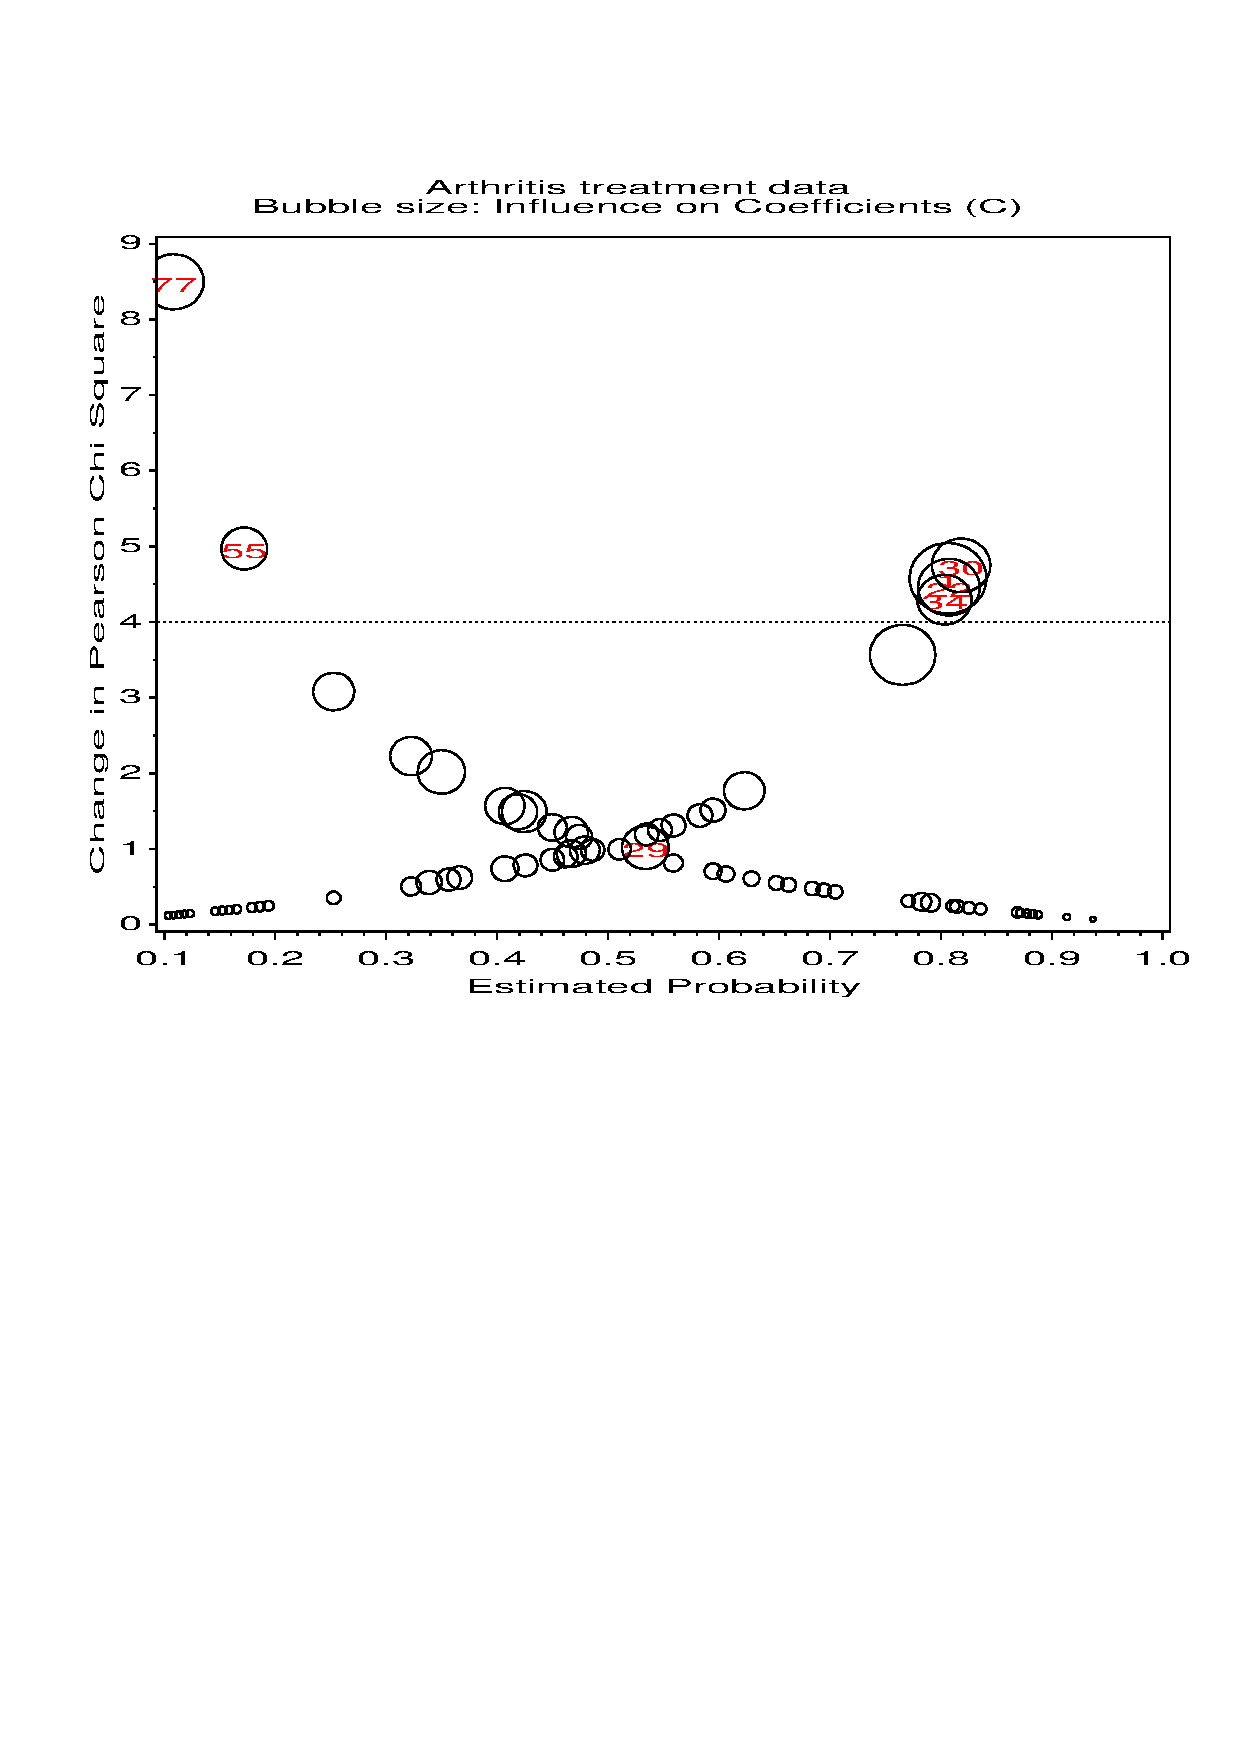
\includegraphics[width=.8\dispwidth,clip]{fig/logist1b1}
 \end{center}

\end{frame}

\begin{frame}
  \frametitle{\macrot{INFLOGIS}: Example}
 \begin{center}
  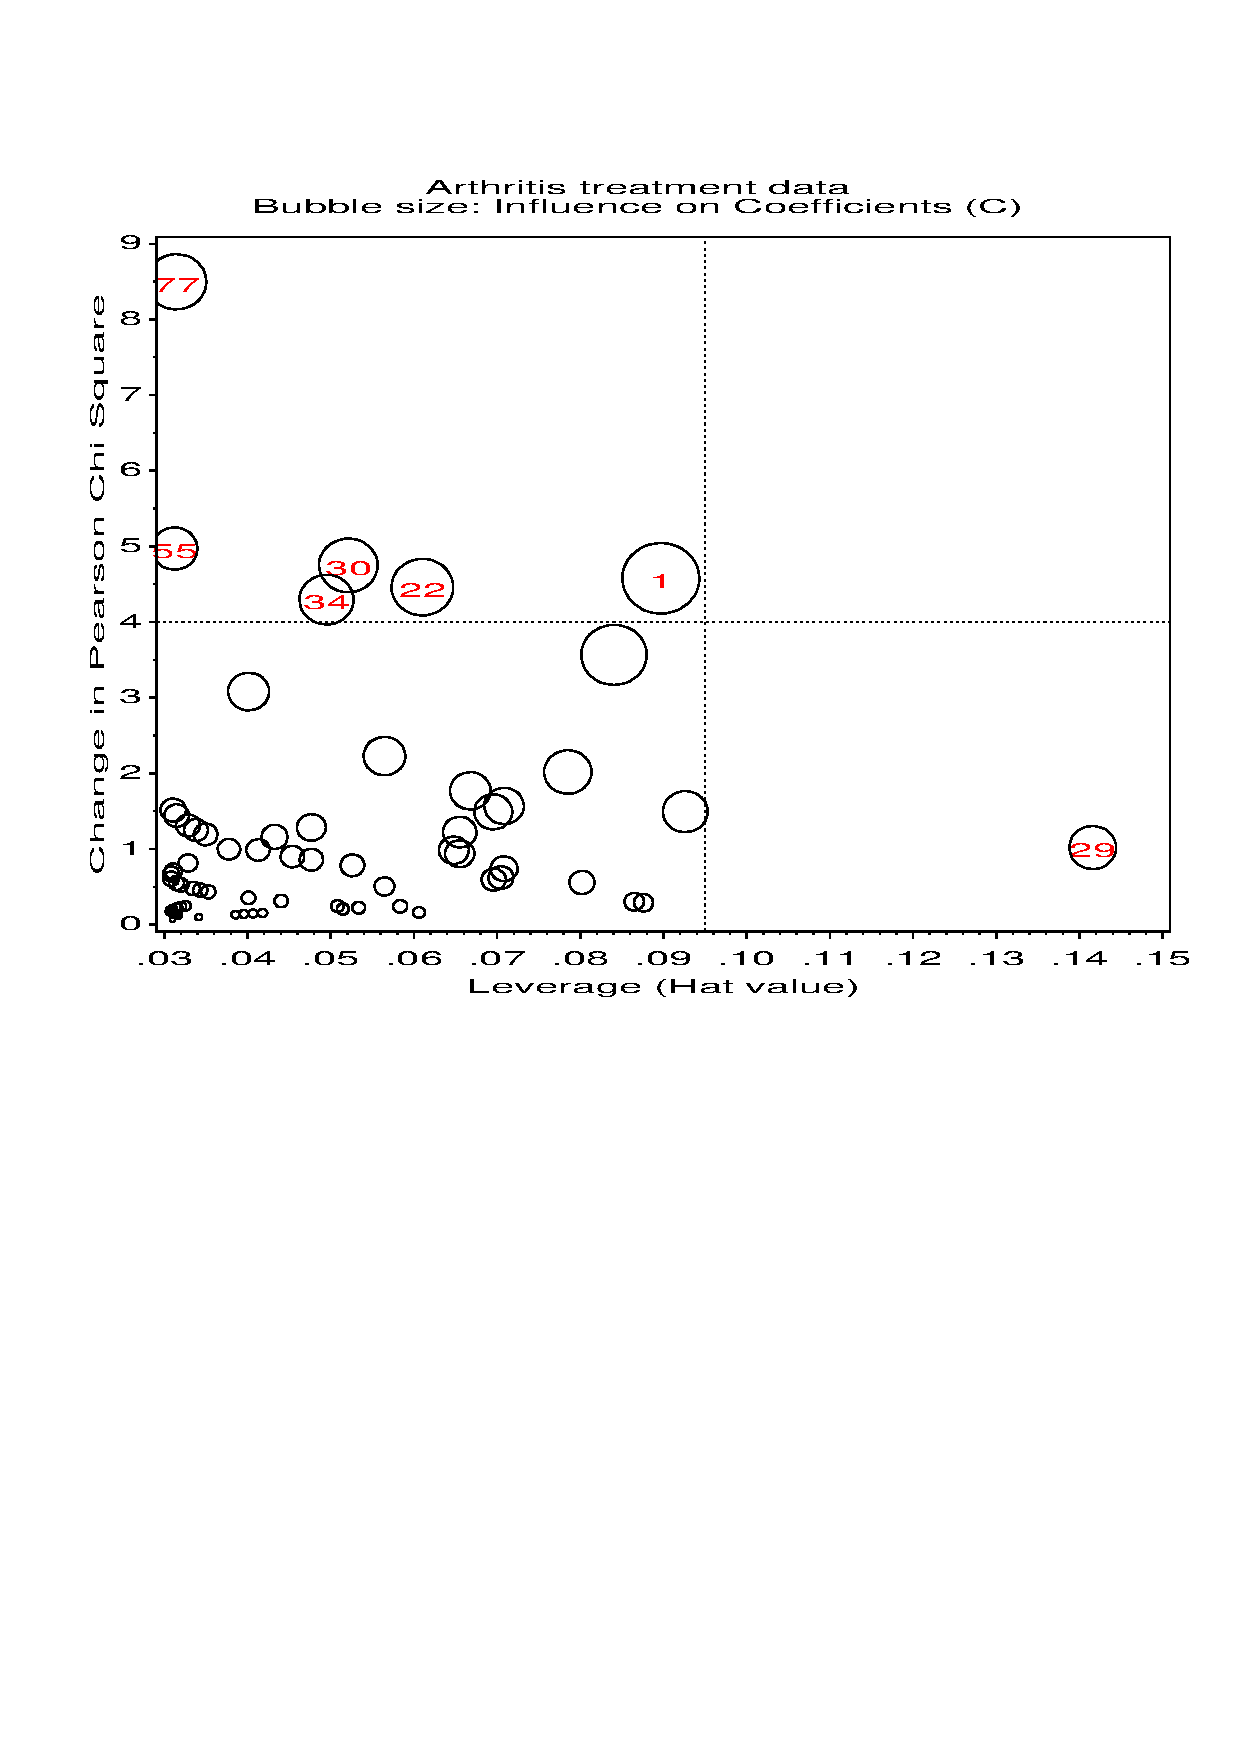
\includegraphics[width=.8\dispwidth,clip]{fig/logist1b2}
 \end{center}

\end{frame}
